\documentclass[handout,xcolor=dvipsnames]{beamer}
\usepackage{multicol}
\usepackage{xy}
\everymath{\displaystyle}
\mode<presentation>
{\usetheme{Warsaw}\setbeamercovered{dynamic}}
\usecolortheme{crane}
\usepackage{beamerfoils}
\pgfdeclareimage[height=1in]{university-logo}{ISULogo}
\logo{\pgfuseimage{university-logo}}
\setbeamertemplate{navigation symbols}{}
\title[\S11]{Section 11\\Binomial probability}
\author{Dr Marcus Bishop}
\subject{Math 104}
\beamerdefaultoverlayspecification{<+->}
\theoremstyle{definition}
\newtheorem{remark}{Remark}
\newtheorem{impact}{Impact}
\newtheorem{situation}{Situation}
\newtheorem{question}{Question}
\usepackage{arev}
\usepackage{tensor}
\newcommand\npr[2]{\tensor[_{#1}]P{_{#2}}}
\newcommand\ncr[2]{\tensor[_{#1}]C{_{#2}}}
\usepackage{cancel}
\newcommand{\hs}{\alert{\varheart}}
\newcommand{\ds}{\alert{\vardiamond}}
\newcommand{\s}{\spadesuit}
\newcommand{\cs}{\clubsuit}
\begin{document}
\begin{frame}\titlepage\end{frame}
\LogoOff

\begin{frame}{Binomial theorem}
\begin{itemize}
\item Recall FOIL method:
\begin{align*}
\left(x+y\right)^2
\only<+->{&=\left(x+y\right)\left(x+y\right)\\}
\only<+->{&=x^2+xy+yx+y^2\\}
\only<+->{&=x^2+2xy+y^2}
\end{align*}
\begin{remark}
\begin{itemize}
\item $\left(x+y\right)^2\alert{\ne}x^2+y^2$
as commonly mistaken
\item Rather $\left(x+y\right)^2=x^2+2xy+y^2$
as shown above
\end{itemize}
\end{remark}
\begin{remark}
\begin{itemize}
\item Order of factors in monomials not important
\item $x^2y=xyx=yx^2$, for example
\item However, numbers of $x$'s and $y$'s important
\end{itemize}
\end{remark}
\end{itemize}
\end{frame}

\begin{frame}
\begin{itemize}
\item Similarly for third power:
\begin{align*}
\left(x+y\right)^3
\only<+->{&=\left(x+y\right)\left(x+y\right)\left(x+y\right)\\}
\only<+->{&=\left(x+y\right)^2\left(x+y\right)\\}
\only<+->{&=\left(x^2+2xy+y^2\right)\left(x+y\right)\\}
\only<+->{&=x^3+x^2y+2xyx+2xy^2+y^2x+y^3\\}
\only<+->{&=x^3+3x^2y+3xy^2+y^3\\}
\only<+->{&=\alert{1}x^3+\alert{3}x^2y+\alert{3}xy^2+\alert{1}y^3}
\end{align*}
\item Similarly for fourth power:
\begin{align*}
\left(x+y\right)^4&=x^4+4x^3y+6x^2y^2+4xy^3+y^4\\
\only<+->{&=\alert{1}x^4+\alert{4}x^3y+\alert{6}x^2y^2
+\alert{4}xy^3+\alert{1}y^4}
\end{align*}
\item Note that coefficients $1,4,6,4,1$ the numbers
in fourth row of Pascal's triangle
\end{itemize}
\end{frame}

\begin{frame}
\begin{itemize}
\item Recall Pascal's triangle:
\[\begin{array}{ccccccccccccc}
&&&&&&1\\
&&&&&1&&1\\
\only<+->{
&&&&1&&2&&1\\}
\only<+->{
&&&1&&3&&3&&1\\}
\only<+->{
&&1&&4&&6&&4&&1\\}
\only<+->{
&1&&5&&10&&10&&5&&1\\}
\only<+->{
1&&6&&15&&20&&15&&6&&1}
\end{array}\]
\item $\ncr{n}{r}=\frac{n!}{\left(n-r\right)!r!}$ the
number in row $n$~position~$r$
(counting from zero)
\item $\ncr{n}{r}$ also the coefficient
of $x^ry^{n-r}$ in expansion of $\left(x+y\right)^n$
\item Thus $\ncr{n}{r}$ called a \alert{binomial coefficient}
\end{itemize}
\end{frame}

\begin{frame}{Connection to probability}
\begin{itemize}
\item You flip coin three times
\item Want to calculate probability of \alert{exactly} two heads
\item Could successfully happen in several ways
\item But how to count them?
\item Start by listing all outcomes:
\[HHH\quad HHT\quad HTH\quad HTT\quad THH\quad THT\quad TTH\quad TTT\]
\item Note that \alert{three} outcomes have exactly two heads:
\[HHH\quad\alert{HHT}\quad\alert{HTH}
\quad HTT\quad\alert{THH}\quad THT\quad TTH\quad TTT\]
\item So $\frac{3}{8}$ the probability of flipping exactly two heads
\end{itemize}
\end{frame}

\begin{frame}
\begin{itemize}
\item But how to calculate without listing outcomes?
\item Two choices ($H$ or $T$) for first flip
\item Two choices for second, two for third
\item So $2\cdot 2\cdot 2=2^3=8$ possible outcomes
\item How many have exactly two heads?
\item Need to select two of three flips to be heads
\item Can choose heads in $\ncr{3}{2}=3$ ways
\item Recall that $HHT,HTH,THH$ the three ways
(not strictly necessary to enumerate)
\item Each of eight outcomes equally likely
\item So $\frac{3}{8}$ the probability of exactly two heads
\end{itemize}
\end{frame}

\begin{frame}{Harder example}
\begin{itemize}
\item Calculate probability of exactly five heads in eight coin tosses
\item Too difficult to enumerate all outcomes
\item Only need \alert{number} of possible outcomes
\item Two choices for first toss, two for second, etc.
\item So $2\cdot 2\cdots 2=2^8=256$ possible outcomes
\item How many have exactly five heads?
\item Need to select five of eight flips to be heads
\item Can be chosen in $\ncr{8}{5}=56$ ways
\item Thus $\frac{56}{256}=\frac{7}{32}$ the probability
of exactly five heads
\end{itemize}
\end{frame}

\begin{frame}
\begin{itemize}
\item More generally $\frac{\ncr{n}{r}}{2^n}$ the probability
of exactly $r$~heads in $n$~coin tosses
\item \dots since $2^n$ possible outcomes, $\ncr{n}{r}$
of which have exactly $r$~heads
\begin{example}
\begin{itemize}
\item You don't know answers to ten-question true/false quiz
\item Calculate probability of correctly guessing exactly eight
\item $2^{10}=1024$ ways to guess
\item $\ncr{10}{8}=45$ ways have exactly eight correct
\item So $\frac{45}{1024}\approx 0.044$ the probability
of exactly eight correct
\end{itemize}
\end{example}
\end{itemize}
\end{frame}

\begin{frame}
\begin{itemize}
\item Similarly
$\frac{\ncr{10}{10}}{2^{10}}\approx 0.0001$
the probability of correctly guessing ten
\item $\frac{\ncr{10}{9}}{2^{10}}\approx 0.0098$
the probability of correctly guessing nine
\item $\frac{\ncr{10}{8}}{2^{10}}\approx 0.044$
the probability of correctly guessing eight (see previous slide)
\item $\frac{\ncr{10}{7}}{2^{10}}\approx 0.1172$
the probability of correctly guessing seven
\item So $0.0001+0.0098+0.044+0.1172=0.1719$
the probability of correctly guessing $7$ or $8$ or $9$ or $10$
\item So $P\left(\text{seven or more correct}\right)=0.1719$
\end{itemize}
\end{frame}

\begin{frame}{Multiple choice quiz}
\begin{itemize}
\item However, life not so simple if quiz questions have
more than two answer choices
\item Suppose quiz has three questions, each with five answer choices
\item Thus, each guess much more likely to be incorrect than correct
\item In contrast, on true/false quiz, each guess as likely
to be correct as incorrect
\end{itemize}
\end{frame}

\begin{frame}
\begin{itemize}
\item Each question has two outcomes:
\begin{itemize}
\item Right (R) with probability $\frac{1}{5}$
\item Wrong (W) with probability $\frac{4}{5}$
\end{itemize}
\item Possible outcomes of quiz:
\[RRR\quad RRW\quad RWR\quad RWW\quad WRR\quad WRW\quad WWR\quad WWW\]
\item In contrast with true/false quiz, outcomes above not equally likely
\item $P\left(RRR\right)=\frac{1}{5}\cdot\frac{1}{5}\cdot\frac{1}{5}
=\frac{1}{125}$
\item $P\left(RRW\right)=\frac{1}{5}\cdot\frac{1}{5}\cdot\frac{4}{5}
=\frac{4}{125}$
\end{itemize}
\end{frame}

\begin{frame}
\begin{itemize}
\item However, $P\left(RRW\right)=\frac{4}{125}$
\alert{not} the probability of correctly guessing two
\item \dots because correctly guessing two can also happen
in other ways, namely $RWR$ and $WRR$
\item $P\left(RWR\right)=\frac{1}{5}\cdot\frac{4}{5}\cdot\frac{1}{5}
=\frac{4}{125}$
\item $P\left(WRR\right)=\frac{4}{5}\cdot\frac{1}{5}\cdot\frac{1}{5}
=\frac{4}{125}$
\item Note that each way to correctly guess two has probability
$\frac{4}{125}$
\item So $P\left(\text{exactly two correct}\right)=3\cdot\frac{4}{125}
=\frac{12}{125}$
\end{itemize}
\end{frame}

\begin{frame}{Binomial probability summary}
\begin{itemize}
\item Suppose same experiment repeated $n$ times
\item Experiment has exactly two outcomes:
\begin{itemize}
\item Success ($S$) with probability $p$
\item Failure ($F$) with probability $1-p$
\end{itemize}
\item Want to calculate probability of exactly $r$~successes
\item Two choices ($S$ or $F$) for first trial, two for second, etc.
\item So $2\cdot 2\cdots 2=2^n$ possible outcomes (although $2^n$
not part of final answer in general)
\item How many have exactly $r$~successes?
\item Need to choose $r$ trials to be $S$
\item Then remaining $n-r$ trials must be $F$
\item $\ncr{n}{r}$ ways to choose $r$ successes,
so $\ncr{n}{r}$ outcomes have exactly $r$~successes
\item Each outcome with $r$~successes has probability
$p^r\left(1-p\right)^{n-r}$
\item So $P\left(\text{exactly $r$ successes}\right)
=\ncr{n}{r}p^r\left(1-p\right)^{n-r}$
\end{itemize}
\end{frame}

\begin{frame}
\begin{example}
\begin{itemize}
\item Probability of correctly guessing exactly seven answers
on ten-question quiz
\item Each question has five answer choices,
so $p=\frac{1}{5}$
\item So $P\left(\text{exactly $7$ correct}\right)
=\ncr{10}{7}\left(\frac{1}{5}\right)^7\left(\frac{4}{5}\right)^3
\only<+->{\approx 0.0008}$
\end{itemize}
\end{example}
\begin{example}
\begin{itemize}
\item Probability of exactly $r$~heads in $n$~coin tosses
\item $P\left(H\right)=\frac{1}{2}=P\left(T\right)$
\item So $P\left(\text{exactly $r$ heads}\right)
=\ncr{n}{r}\left(\frac{1}{2}\right)^r\left(\frac{1}{2}\right)^{n-r}
=\frac{\ncr{n}{r}}{2^n}$
\item Agrees with calculation above
\end{itemize}
\end{example}
\end{frame}

\begin{frame}{Basketball example}
\begin{multicols}{2}
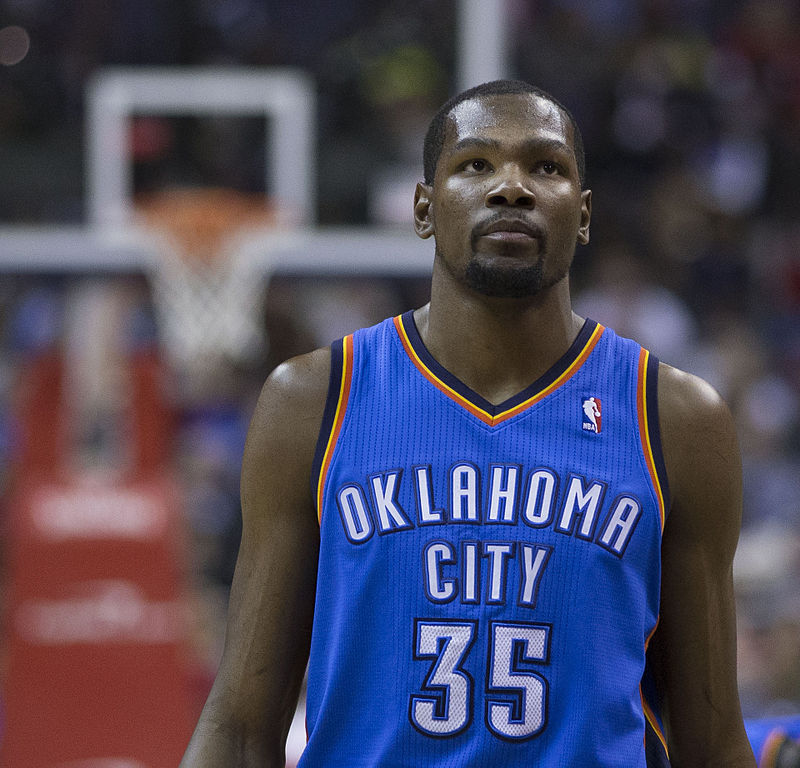
\includegraphics[scale=.75]{KevinDurant}
\begin{itemize}
\item Kevin Durant made 679 of 750 attempted free-throws
in 2012--2013 season with Oklahoma City Thunder
\item Suppose Durant awarded three free-throws
\item Calculate probability he makes exactly two
\item $p=\frac{679}{750}\approx 0.9053$ the probability
each time
\item So $P\left(\text{exactly two}\right)
=\ncr{3}{2}\left(0.9053\right)^2\left(0.0947\right)^1=0.2328$
\end{itemize}
\end{multicols}
\end{frame}

\begin{frame}
\begin{itemize}
\item $P\left(\text{exactly three}\right)
=\ncr{3}{3}\left(0.9053\right)^3\left(0.0947\right)^0=0.742$
\item $P\left(\text{exactly two}\right)
=\ncr{3}{2}\left(0.9053\right)^2\left(0.0947\right)^1=0.2328$
(see previous slide)
\item $P\left(\text{exactly one}\right)
=\ncr{3}{1}\left(0.9053\right)^1\left(0.0947\right)^2=0.0244$
\item $P\left(\text{exactly zero}\right)
=\ncr{3}{0}\left(0.9053\right)^0\left(0.0947\right)^3=0.0008$
\item More realistic question: probability he makes two or more?
\item $P\left(\text{at least two}\right)=0.742+0.2328=0.9748$
\item Note that $0.742+0.2328+0.0244+0.0008=1$
\item Indeed, $1=\left(p+\left(1-p\right)\right)^3
\only<+->{=
\ncr{3}{0}p^0\left(1-p\right)^3
+\ncr{3}{1}p^1\left(1-p\right)^2
+\ncr{3}{2}p^2\left(1-p\right)^1
+\ncr{3}{3}p^3\left(1-p\right)^0}$
\end{itemize}
\end{frame}

\begin{frame}{Probability distribution}
\begin{itemize}
\item Calculation of $P\left(\text{exactly $r$ successes}\right)$
for every $0\le r\le n$ called the \alert{probability distribution}
of experiment
\begin{example}
\[\begin{array}{r|rrrr}
r&0&1&2&3\\\hline
P\left(r\right)
&0.0008&0.0244&0.2328&0.742
\end{array}\]
the distribution of basketball example
\end{example}
\item Outcomes $r=0,r=1,\ldots,r=n$
mutually exclusive
\item Exactly one must occur
\item So $1=
P\left(0\right)+P\left(1\right)+\cdots+P\left(n\right)$
\end{itemize}
\end{frame}

\begin{frame}{Quality control for batteries (Example 2)}
\begin{itemize}
\item Battery manufacturer knows that $0.4$ percent of batteries
defective
\item If package contains ten batteries, calculate probability
distribution of number of defective batteries
\item $p=0.004$ the probability random battery defective
\item So $P\left(\text{exactly $0$ defective}\right)
=\ncr{10}{0}\left(0.004\right)^0\left(0.996\right)^{10}\approx 0.9607$
\item So $P\left(\text{exactly $1$ defective}\right)
=\ncr{10}{1}\left(0.004\right)^1\left(0.996\right)^9\approx 0.0389$
\end{itemize}
\end{frame}
\begin{frame}
\begin{itemize}
\item Probability distribution for number of defective batteries:
\[\begin{array}{rr}
r&P\left(\text{Exactly $r$ defective}\right)\\\hline
0&0.9607\\
1&0.0389\\
2&0.0007\\
3&0.000007\\
4&0.00000005\\
5&0.0000000002\\
6&0.0000000000008\\
7&0.000000000000001\\
8&0.000000000000000002\\
9&0.000000000000000000002\\
10&0.000000000000000000000001
\end{array}\]
\item Want to calculate $P\left(\text{One or more defective}\right)$
\item Too cumbersome to add $0.0389+0.0007+\cdots$
\item Easier: $P\left(\text{One or more defective}\right)=
1-0.960712373502810=0.0392876264971900$
\end{itemize}
\end{frame}
\end{document}
